% Created 2022-10-18 Tue 15:19
% Intended LaTeX compiler: pdflatex
\documentclass[11pt]{article}
\usepackage[utf8]{inputenc}
\usepackage[T1]{fontenc}
\usepackage{graphicx}
\usepackage{longtable}
\usepackage{wrapfig}
\usepackage{rotating}
\usepackage[normalem]{ulem}
\usepackage{amsmath}
\usepackage{amssymb}
\usepackage{capt-of}
\usepackage{hyperref}
\AddToHook{cmd/section/before}{\clearpage}
%\AddToHook{cmd/subsection/before}{\clearpage}
\graphicspath{{../../books/}}
% TIPS
% \substack{a\\b} for multiple lines text





% pdfplots will load xolor automatically without option
\usepackage[dvipsnames]{xcolor}

\usepackage{forest}
% two-line text in node by [two \\ lines]
% \begin{forest} qtree, [..] \end{forest}
\forestset{
  qtree/.style={
    baseline,
    for tree={
      parent anchor=south,
      child anchor=north,
      align=center,
      inner sep=1pt,
    }}}
%\usepackage{flexisym}
% load order of mathtools and mathabx, otherwise conflict overbrace

\usepackage{mathtools}
%\usepackage{fourier}
\usepackage{pgfplots}
\usepackage{amsthm, mathabx,  amsmath, commath}
\usepackage{amsfonts}

\usepackage{empheq}
\usepackage{tikz}
\usetikzlibrary{arrows.meta}
\usepackage[most]{tcolorbox}

\newtheorem{theorem}{Theorem}[section]
\newtheorem{definition}{Definition}[section]
\newtheorem{corollary}{Corollary}[section]
\newtheorem{example}{Example}[section]
\newtheorem{lemma}{Lemma}[section]
\newtheorem{proposition}{Proposition}[section]

\newcommand{\bl}[1] {\boldsymbol{#1}}
\newcommand{\Wt}[1] {\stackrel{\sim}{\smash{#1}\rule{0pt}{1.1ex}}}
\newcommand{\wt}[1] {\widetilde{#1}}


%For boxed texts in align, use Aboxed{}
%otherwise use boxed{}

\DeclareMathSymbol{\widehatsym}{\mathord}{largesymbols}{"62}
\newcommand\lowerwidehatsym{%
  \text{\smash{\raisebox{-1.3ex}{%
    $\widehatsym$}}}}
\newcommand\fixwidehat[1]{%
  \mathchoice
    {\accentset{\displaystyle\lowerwidehatsym}{#1}}
    {\accentset{\textstyle\lowerwidehatsym}{#1}}
    {\accentset{\scriptstyle\lowerwidehatsym}{#1}}
    {\accentset{\scriptscriptstyle\lowerwidehatsym}{#1}}
}

\usepackage{graphicx}
    
% text on arrow for xRightarrow
\makeatletter
%\newcommand{\xRightarrow}[2][]{\ext@arrow 0359\Rightarrowfill@{#1}{#2}}
\makeatother


\def \bx {\boldsymbol{x}}
\def \ba {\boldsymbol{a}}
\def \bI {\boldsymbol{I}}
\def \bt {\boldsymbol{t}}
\def \bb {\boldsymbol{b}}
\def \bA {\boldsymbol{A}}
\def \bX {\boldsymbol{X}}
\def \bu {\boldsymbol{u}}
\def \bS {\boldsymbol{S}}
\def \bZ {\boldsymbol{Z}}
\def \bz {\boldsymbol{z}}
\def \by {\boldsymbol{y}}
\def \bw {\boldsymbol{w}}
\def \bT {\boldsymbol{T}}
\def \bS {\boldsymbol{S}}
\def \bm {\boldsymbol{m}}
\def \bW {\boldsymbol{W}}
\def \bY {\boldsymbol{Y}}
\def \bH {\boldsymbol{H}}
\def \blambda {\boldsymbol{\lambda}}
\def \bPhi {\boldsymbol{\Phi}}
\def \btheta {\boldsymbol{\theta}}
\def \bmu {\boldsymbol{\mu}}
\def \bphi {\boldsymbol{\phi}}
\def \bSigma {\boldsymbol{\Sigma}}
\def \lb {\left\{}
\def \rb {\right\}}
\def \caln {\mathcal{N}}
\def \dissum {\displaystyle\Sigma}
\def \dispro {\displaystyle\prod}
\def \E {\mathbb{E}}
\def \Q {\mathbb{Q}}
\def \V {\mathbb{V}}
\def \R {\mathbb{R}}
\def \calq {\mathcal{Q}}
\def \calg {\mathcal{G}}
\def \caln {\mathcal{N}}
\def \calr {\mathcal{R}}
\def \calm {\mathcal{M}}
\def \calc {\mathcal{C}}
\def \bcup {\bigcup}

\makeindex
\usepackage{minted}
\renewcommand*{\proofname}{Solution}
\let\OldTexttt\texttt
\renewcommand{\texttt}[1]{\OldTexttt{\color{MidnightBlue} #1}}
\author{wu}
\date{\today}
\title{Competitive programming}
\hypersetup{
 pdfauthor={wu},
 pdftitle={Competitive programming},
 pdfkeywords={},
 pdfsubject={},
 pdfcreator={Emacs 28.0.92 (Org mode 9.6)}, 
 pdflang={English}}
\begin{document}

\maketitle
\tableofcontents


\section{Dynamic Programming}
\label{sec:orgc8d194f}
\subsection{General}
\label{sec:orge0fe9e4}
\begin{problem}[\href{https://leetcode.cn/problems/find-all-good-indices/}{LeetCode: Find All Good Indices}]
You are given a \emph{0-indexed} integer array nums of size \(n\) and a positive integer \(k\).

We call an index \(i\) in the range \(k\le i< n-k\) good if the following conditions are satisfied:
\begin{itemize}
\item The \(k\) elements that are just before the index \(i\) are in non-increasing order.
\item The \(k\) elements that are just after the index \(i\) are in non-decreasing order.
\end{itemize}

Return an array of all good indices sorted in increasing order.
\end{problem}

\begin{proof}
For \(j\), suppose the non-increasing elements before \(j\) (including \(j\)) is \(left_j\), the
non-decreasing elements after \(j\) (including \(j\)) is \(right_j\), then \(i\) is good iff
\(left_{i-1}\ge k\) and \(right_{i+1}\ge k\)
\end{proof}

\begin{problem}[\href{https://leetcode.cn/problems/get-kth-magic-number-lcci/}{LeetCode: Get Kth Magic Number}]
Design an algorithm to find the kth number such that the only prime factors are 3, 5, and 7.
Note that 3, 5, and 7 do not have to be factors, but it should not have any other prime factors.
For example, the first several multiples would be (in order) 1, 3, 5, 7, 9, 15, 21.
\end{problem}

\begin{proof}
We can use heap: for each element \(x\) took out, add \(3x,5x,7x\) into the heap. Also we need
to eliminate the duplicates

Define \(dp[i]\) is the \(i\)th number, so \(dp[1]=1\), and let \(p_3=p_5=p_7=1\) initially, then
for \(2 \le i\le k\)
\begin{equation*}
dp[i]=\min(dp[p_3]\cdot 3, dp[p_5]\cdot 5, dp[p_7]\cdot 7)
\end{equation*}
and increment the corresponding \(p_k\) where \(k\in\{3,5,7\}\)
\end{proof}

\begin{problem}[\href{https://leetcode.cn/problems/remove-boxes/}{LeetCode: Remove Boxes}]
You are given several boxes with different colors represented by different positive numbers.

You may experience several rounds to remove boxes until there is no box left. Each time you can
choose some continuous boxes with the same color (i.e., composed of \(k\) boxes, \(k\ge 1\)), remove
them and get \(k^2\) points.

\emph{Return the maximum points you can get.}
\end{problem}

\begin{proof}
Let \(dp(l,r,k)\) denote the maximum points we can get in boxes \([l,r]\) if we have extra \(k\)
boxes which is the same color with \(boxes[l]\) in the left side.

For example, if \texttt{boxes=[3,3,1,3,3]}, then \(dp(3,4,2)\) is the maximum we can get in \texttt{boxes[3,4]} if
we have extra 2 boxes the same color with \texttt{boxes[3]} in the left side

Since \((a+b)^2>a^2+b^2\) where \(a>0,b>0\), it's better to greedy to remove all contiguous boxes
of the same color, instead of split them. So we increase both \(l\) and \(k\) while
\texttt{boxes[l+1]==boxes[l]}

Now we have some options:
\begin{itemize}
\item remove all boxes which has the same color with boxes \(l\), total points we can get is
\(dp(l+1,r,0)+(k+1)^2\)
\item merge non-contiguous boxes of the same color together, by
\begin{itemize}
\item find the index \(j\) where \(l+1\le j\le r\) so that \texttt{boxes[j]==boxes[l]}
\item total points we can get is \(dp(j,r,k+1)+dp(l+1,j-1,0)\)
\end{itemize}
\end{itemize}

\begin{figure}[htbp]
\centering
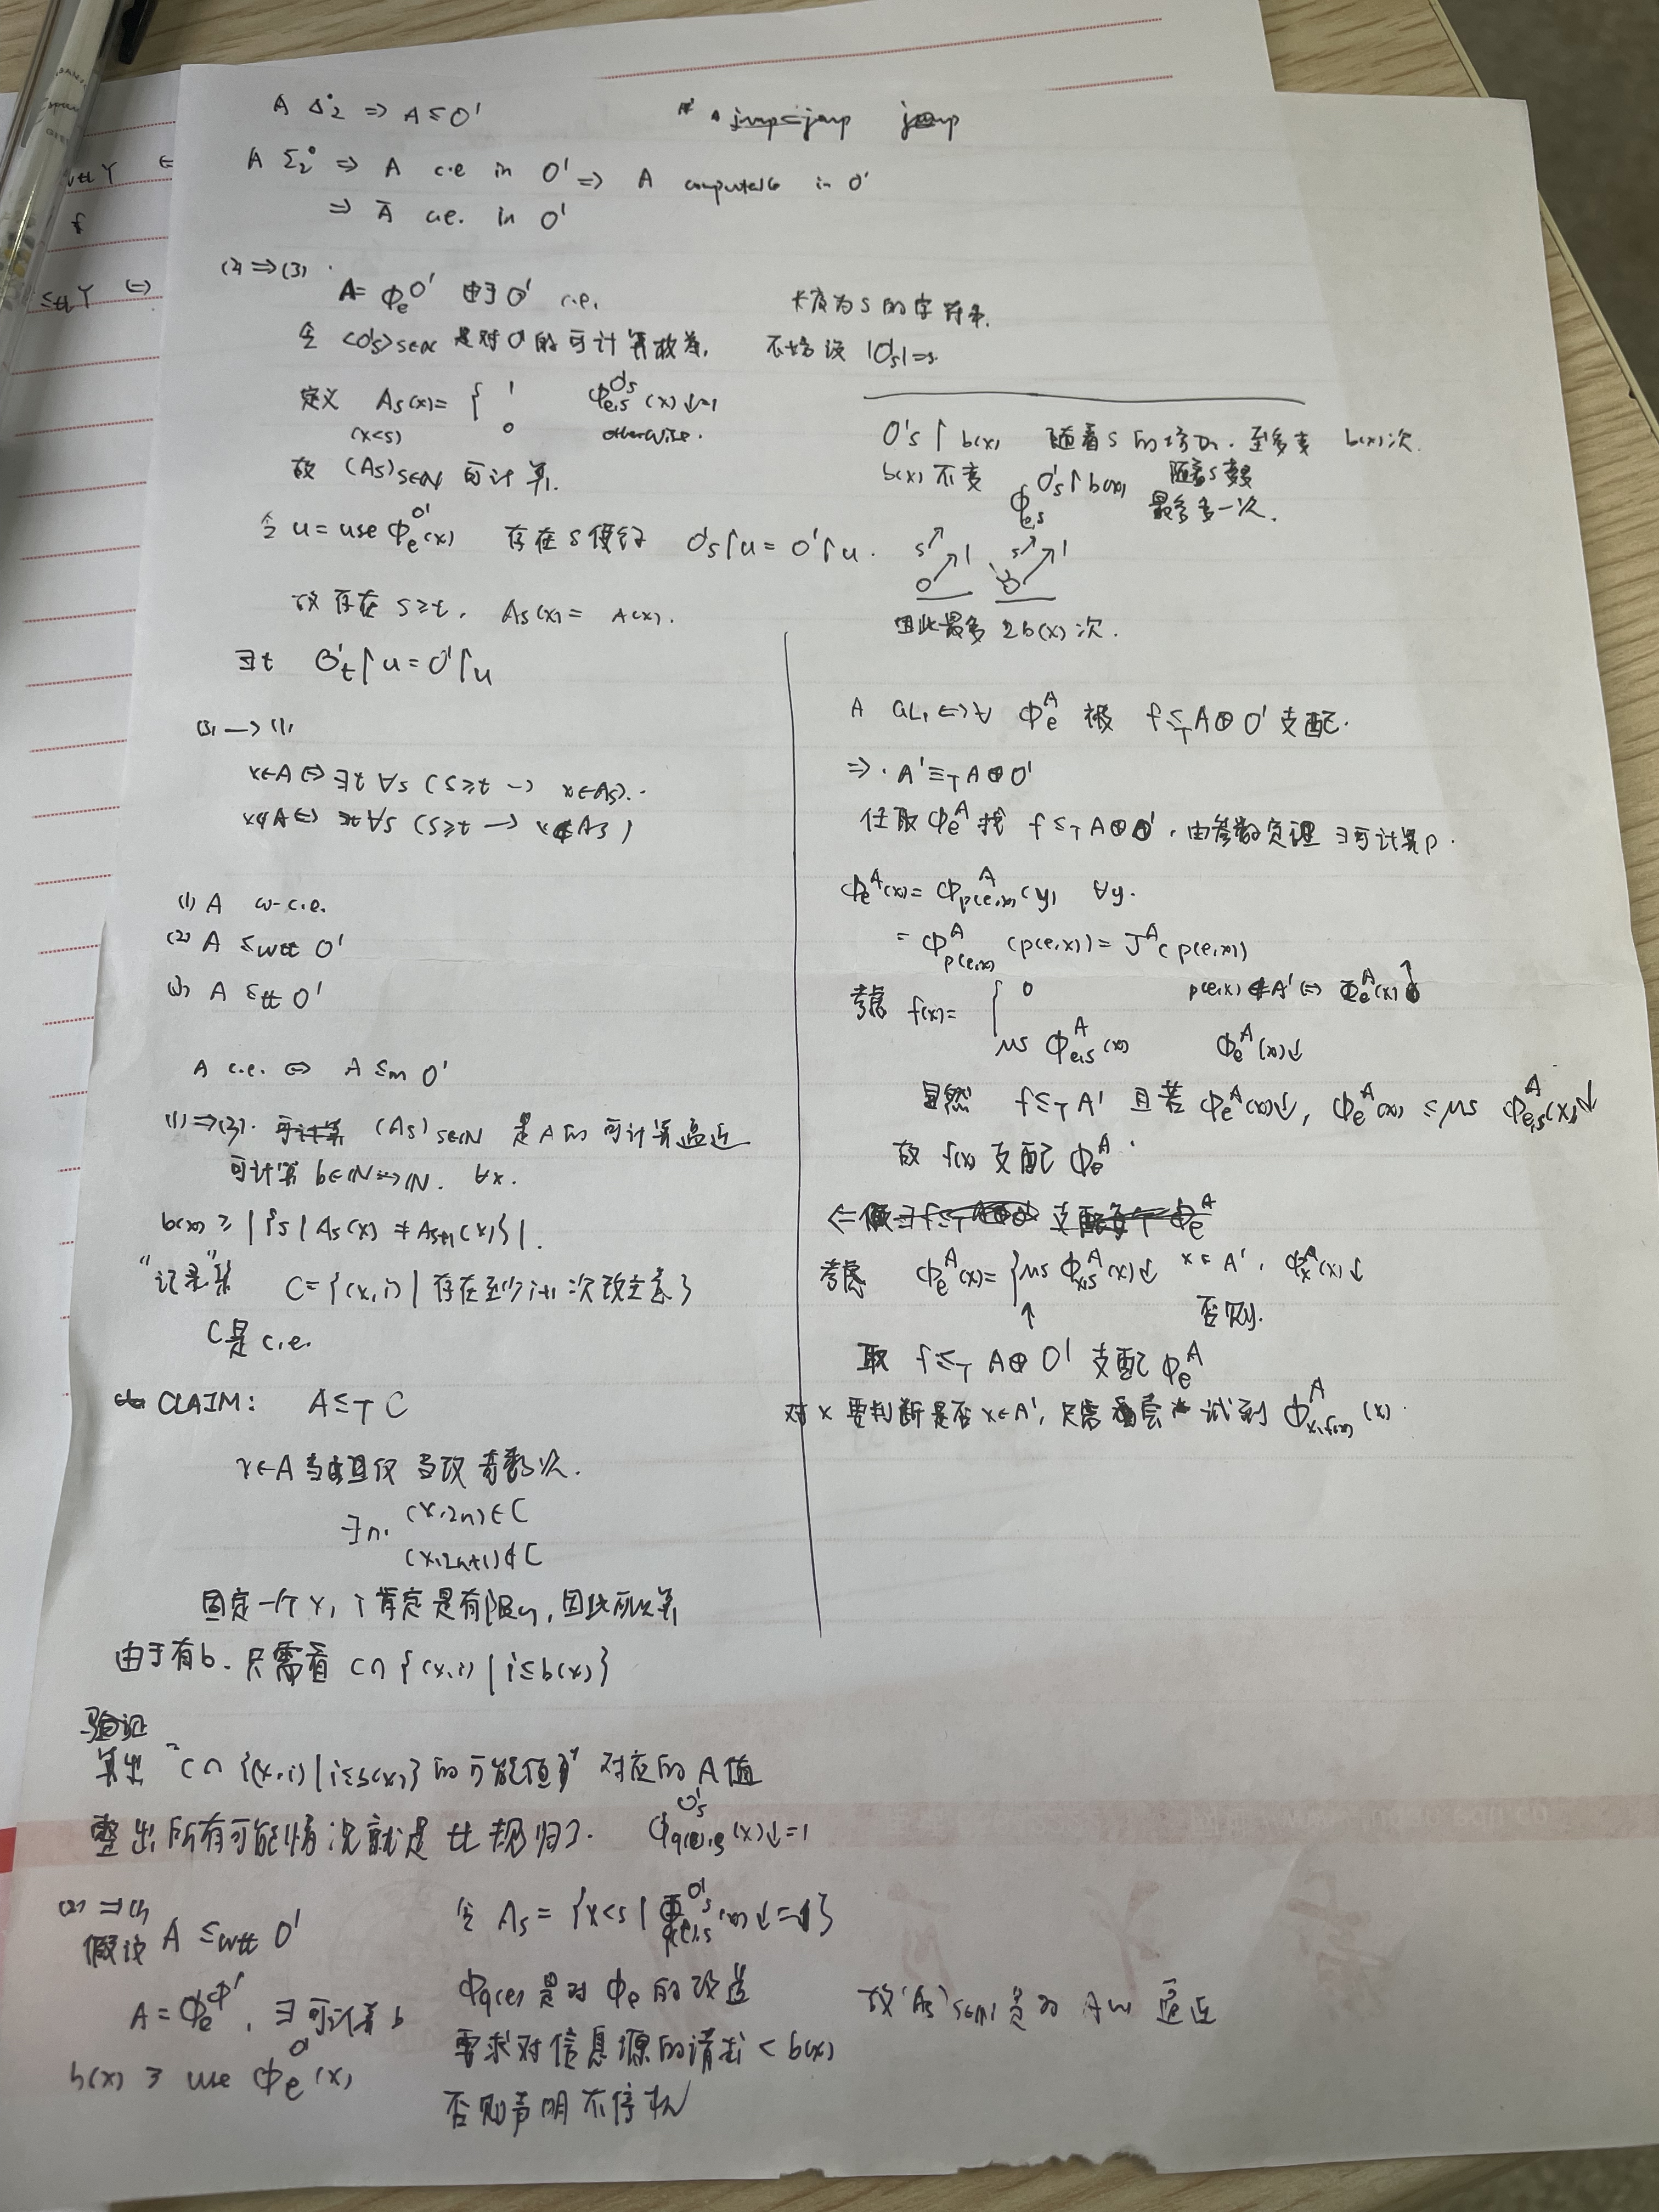
\includegraphics[width=.6\textwidth]{../images/cp/1.png}
\label{}
\end{figure}
\end{proof}

\begin{problem}[\href{https://leetcode.cn/problems/k-inverse-pairs-array/}{LeetCode: K Inverse Pairs Array}]
For an integer array nums, an \textbf{inverse pair} is a pair of integers \((i,j)\)
where \(0\le i<j<len(nums)\) and \(nums[i]>nums[j]\)

Given two integers \(n\) and \(k\), return the number of different arrays consist of numbers
from 1 to \(n\) such that there are exactly \(k\) inverse pairs. Since the answer can be huge,
return it modulo \(10^9+7\).
\end{problem}

\begin{proof}
Let \(f(i,j)\) denote the number of different arrays consisting of numbers from 1 to \(i\) s.t.
there are exactly \(j\) inverse pairs.

Suppose we fix \(k\) as the last element of the array, then the number of inverse pairs is the sum of
\begin{itemize}
\item the inverse pairs between \(k\) and other numbers
\item the inverse pairs among other numbers
\end{itemize}

The first part is \(i-k\), therefore the second part should be \(j-(i-k)\).
\begin{equation*}
f(i,j)=\sum_{k=1}^if(i-1,j-(i-k))=\sum_{k=0}^{i-1}f(i-1,j-k)
\end{equation*}
But the above formula's complexity is \(O(n^2k)\).

Note that
\begin{align*}
f(i,j-1)&=\sum_{k=0}^{i-1}f(i-1,j-1-k)\\
f(i,j)&=\sum_{k=0}^{i-1}f(i-1,j-k)
\end{align*}
Therefore
\begin{equation*}
f(i,j)=f(i,j-1)-f(i-1,j-i)+f(i-1,j)
\end{equation*}
\end{proof}

\begin{problem}[\href{https://leetcode.cn/problems/minimum-swaps-to-make-sequences-increasing/}{LeetCode: Minimum Swaps To Make Sequences Increasing}]
You are given two integer arrays of the same length \(nums1\) and \(nums2\). In one operation, you are
allowed to swap \(nums1[i]\) with \(nums2[i]\).

For example, if \(nums1 = [1,2,3,8]\), and \(nums2 = [5,6,7,4]\), you can swap the element at \(i = 3\) to
obtain \(nums1 = [1,2,3,4]\) and \(nums2 = [5,6,7,8]\).

Return the minimum number of needed operations to make \(nums1\) and \(nums2\) strictly increasing. The
test cases are generated so that the given input always makes it possible.

An array arr is strictly increasing if and only if \(arr[0] < arr[1] < arr[2] <\dots < arr[arr.length - 1]\)
\end{problem}

\begin{proof}
For each \(i\), one of the following is true
\begin{enumerate}
\item \(nums_1[i]>nums_1[i-1]\) and \(nums_2[i]>nums_2[i-1]\)
\item \(nums_1[i]>nums_2[i-1]\) and \(nums_2[i]>nums_1[i-1]\)
\end{enumerate}

Use \(dp[i][0]\) to denote the minimum number of needed operations for \([0,i]\) and we don't do
the exchange at \(i\). Use \(dp[i][1]\) to denote the number that we exchange at \(i\).

Case \(1\wedge \neg2\):
\begin{equation*}
\begin{cases}
dp[i][0]=dp[i-1][0]\\
dp[i][1]=dp[i-1][1]+1\\
\end{cases}
\end{equation*}

Case \(\neg1\wedge 2\):
\begin{equation*}
\begin{cases}
dp[i][0]=dp[i-1][1]\\
dp[i][1]=dp[i-1][0]+1
\end{cases}
\end{equation*}

Case \(1\wedge 2\):
\begin{equation*}
\begin{cases}
dp[i][0]=\min\{dp[i-1][0],dp[i-1][1]\}\\
dp[i][1]=\min\{dp[i-1][1],dp[i-1][0]\}+1
\end{cases}
\end{equation*}

and we set \(dp[0][0]=dp[0][1]=1\)
\end{proof}

\begin{problem}[\href{https://leetcode.cn/problems/count-ways-to-build-rooms-in-an-ant-colony/}{LeetCode: Count Ways to Build Rooms i nan Ant Colony}]
You are an ant tasked with adding n new rooms numbered \(0\) to \(n-1\) to your colony. You are given
the expansion plan as a \(0\)-indexed integer array of length \(n\), \(prevRoom\), where \(prevRoom[i]\)
indicates that you must build room \(prevRoom[i]\) before building room \(i\), and these two rooms must
be connected directly. Room \(0\) is already built, so \(prevRoom[0]=-1\). The expansion plan is given
such that once all the rooms are built, every room will be reachable from room \(0\).

You can only build one room at a time, and you can travel freely between rooms you have already
built only if they are connected. You can choose to build any room as long as its previous
room is already built.

Return the number of different orders you can build all the rooms in. Since the answer may be
large, return it modulo \(10^9 + 7\).

Every room is reachable from room \(0\) once all the rooms are built.
\end{problem}

\begin{problem}[]
Suppose there are \(a_0\) 0's, \(a_1\) 1's, \(\dots\), \(a_{n-1}\) \(n-1\)'s, then the number of
different plan to put them in a row is
\begin{equation*}
\frac{(a_0+\dots+a_{n-1})!}{a_0!\cdot a_1!\cdot\dots\cdot a_{n-1}!}
\end{equation*}

\(a^{\varphi(m)}\equiv 1\mod m\), when \(p\) is prime, we have \(a^{p-1}\equiv 1\mod p\)

Define \(f(i)\) to be the number of different topological sort for the subtree with the
root \(i\). Suppose \(i\) has child \(c_{i,0},\dots,c_{i,k}\), and let \(cnt(i)\) denote the number of
nodes in the subtree, then
\begin{equation*}
f(i)=\prod_cf(c)\times\frac{(cnt(i)-1)!}{\prod_ccnt(c)!}
\end{equation*}
\end{problem}

\begin{problem}[\href{https://leetcode.cn/problems/valid-permutations-for-di-sequence/}{LeetCode: Valid Permutations for DI sequence}]
You are given a string s of length \(n\) where \(s[i]\) is either:
\begin{itemize}
\item 'D' means decreasing, or
\item 'I' means increasing.
\end{itemize}
A permutation perm of \(n + 1\) integers of all the integers in the range \([0, n]\) is called a valid
permutation if for all valid \(i\):
\begin{itemize}
\item If \(s[i]='D'\), then \(perm[i] > perm[i + 1]\), and
\item If \(s[i] == 'I'\), then \(perm[i] < perm[i + 1]\).
\end{itemize}
Return the number of valid permutations perm. Since the answer may be large, return it modulo \(10^9 + 7\).
\end{problem}

\begin{proof}
Define o\(dp(i,j)\) to be the number of possible permutations of first \(i+1\) digits where
the \(i+1\)th digit is \(j+1\)th smallest in the rest of unused digits

Let's see an example of ``DID''
\begin{center}
  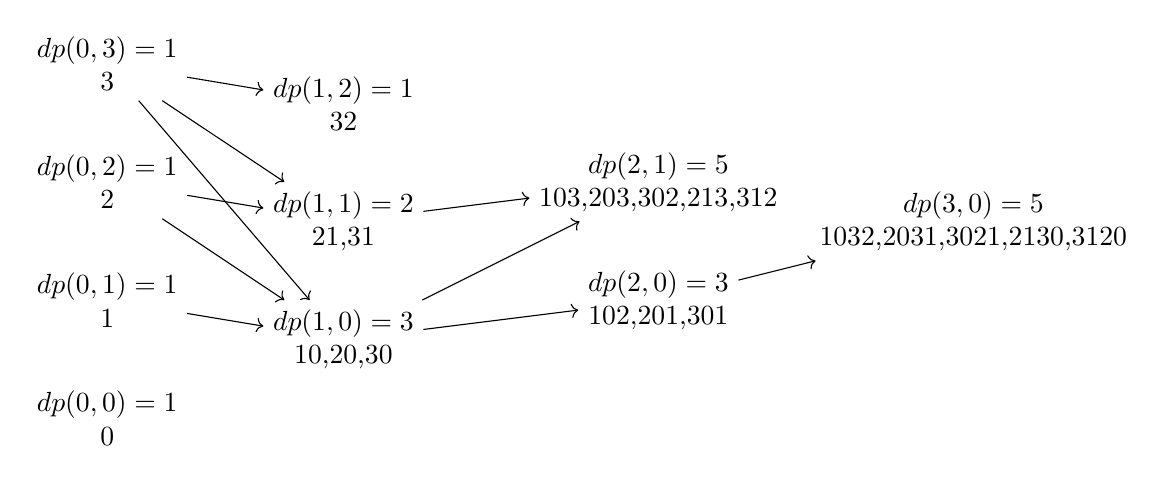
\begin{tikzpicture}[every text node part/.style={align=center}]
    \node (00) at (0,0) {\(dp(0,0)=1\) \\ 0};
    \node (01) at (0,1.5) {\(dp(0,1)=1\) \\ 1};
    \node (02) at (0,3) {\(dp(0,2)=1\) \\ 2};
    \node (03) at (0,4.5) {\(dp(0,3)=1\) \\ 3};
    \node (10) at (3,1) {\(dp(1,0)=3\) \\ 10,20,30};
    \node (11) at (3,2.5) {\(dp(1,1)=2\) \\ 21,31};
    \node (12) at (3,4) {\(dp(1,2)=1\) \\ 32};
    \node (20) at (7,1.5) {\(dp(2,0)=3\) \\ 102,201,301};
    \node (21) at (7,3) {\(dp(2,1)=5\) \\ 103,203,302,213,312};
    \node (30) at (11,2.5) {\(dp(3,0)=5\) \\ 1032,2031,3021,2130,3120};
    \draw[->] (01) to (10);
    \draw[->] (02) to (10);
    \draw[->] (03) to (10);
    \draw[->] (02) to (11);
    \draw[->] (03) to (11);
    \draw[->] (03) to (12);
    \draw[->] (10) to (20);
    \draw[->] (10) to (21);
    \draw[->] (11) to (21);
    \draw[->] (20) to (30);
  \end{tikzpicture}
\end{center}
\end{proof}

\begin{problem}[\href{https://leetcode.cn/problems/distinct-subsequences-ii/}{LeetCode: Distinct Subsequences \rom{2}}]
Given a string \(s\), return the number of distinct non-empty subsequences of \(s\). Since the answer
may be very large, return it modulo \(10^9 + 7\).

A subsequence of a string is a new string that is formed from the original string by deleting
some (can be none) of the characters without disturbing the relative positions of the remaining
characters. (i.e., ``ace'' is a subsequence of ``abcde'' while ``aec'' is not.
\end{problem}

\begin{proof}
Define \(F(i)\) to be the subsequences ends in character \(s[i]\), and \(f(i)=\abs{F(i)}\)

How do we eliminate the duplicates? Note that if \(s[i]=s[j]\) and \(i<j\),
then \(F(i)\subseteq F(j)\), therefore for each character, we only need to care about the last appearance.
\begin{equation*}
f(i)=1+\sum_{0\le k<26,last[k]\neq-1}f(last[k])
\end{equation*}

Note that we only needs 26 values, define \(g[26]\), then
\begin{equation*}
g(c)=1+\sum_{i=0}^{25}g(i)
\end{equation*}
Then, we only need to store \(total=\sum g(i)\).
\end{proof}



\subsection{Digit DP}
\label{sec:org7e78ed9}
\begin{problem}[LeetCode 788: Rotated Digits]
An integer x is a \textbf{good} if after rotating each digit individually by 180 degrees, we get a valid
number that is different  from x. Each digit must be rotated - we cannot choose to leave it alone.

A number is valid if each digit remains a digit after rotation. For example:
\begin{itemize}
\item 0, 1, and 8 rotate to themselves,
\item 2 and 5 rotate to each other (in this case they are rotated in a different direction, in other
words, 2 or 5 gets mirrored)
\item 6 and 9 rotate to each other, and
\item the rest of the numbers do not rotate to any other number and become invalid.
\end{itemize}

Given an integer n, return the number of good integers in the range [1, n].
\end{problem}

\begin{proof}
Given \(n\).
Let \(f(pos,bound,diff)\) be the number of good numbers satisfying
\begin{enumerate}
\item Only consider \(pos\)th digit and \(pos\) starts from left, which means 0th digit is the
highest digit. And we assume the first \(pos-1\)
digits are fixed
\item If digits in \([0,pos-1]\) are first \(pos\) digits of \(n\), then \(bound\) is \texttt{true}
\item If digits in \([0,pos-1]\) has at least one 2/5/6/9, then \(diff\) is \texttt{true}
\end{enumerate}

Therefore the answer is \(f(0, true, false)\), and the transition formula is
\begin{equation*}
f(pos,bound,diff)=\sum f(pos+1,bound',diff')
\end{equation*}
\begin{itemize}
\item \(bound'\) is true iff \(bound\) is true and the digit we choose is the \(pos\)th digit
of \(n\)
\item \(diff'\) is true iff \(diff\) is true or we chose 2/5/6/9
\end{itemize}
\end{proof}

\begin{problem}[\href{https://leetcode.cn/problems/numbers-at-most-n-given-digit-set/}{LeetCode: Numbers at most N given digit set}]
Given an array of digits which is sorted in non-decreasing order. You can write numbers using
each \(digits[i]\) as many times as we want. For example, if digits = ['1','3','5'], we may write
numbers such as '13', '551', and '1351315'.

Return the number of positive integers that can be generated that are less than or equal to a
given integer \(n\).
\end{problem}

\begin{proof}
Suppose we have \(m\) digits.

Define \(dp(i,0)\) to be the number of different number in \(i\) digits that is less than the
first \(i\) digits of \(n\), and \(dp(i,1)\) to be the number of \(i\) digits that is equal to
the first \(i\) digits of \(n\).

Let \(C(i)\) to be the number of digits that is less than \(i\)th digit of \(n\). Then
\begin{equation*}
dp(i,0)=
\begin{cases}
C(i)&i=1\\
m+dp(i-1,0)\times m+dp(i-1,1)\times C(i)&i>1
\end{cases}
\end{equation*}
where \(dp(0,0)=0\) and \(dp(0,1)=1\)
\end{proof}

\section{Graph}
\label{sec:orgc49dbf6}
\subsection{Tree}
\label{sec:org9fe9787}
\begin{problem}[\href{https://leetcode.cn/problems/hSRGyL/}{LeetCode: Navigation Device}]
Given a binary tree \(T\), find minimum number of nodes (device) \(n_1,\dots,n_k\) s.t. for each node \(m\) in
tree, \((d_1,\dots,d_k)\) is unique where \(d_i\) is the distance between \(m\) and \(n_i\).
\end{problem}

\begin{proof}
Observation: Given a subtree of the form
\begin{center}\begin{tikzpicture}[level distance=23pt,sibling distance=20pt]
\Tree
[.​
        [.1
            [.2 \edge[roof]; {} ]
            [.3 \edge[roof]; {} ]
        ]
]
\end{tikzpicture}\end{center}
Then there are at least two device on subtree 2, subtree 3 and parent of 1.

Therefore if we know that ancestors of 1 have device and 1's two childs don't have device, we
should put a device in either 2 or 3.

Now since we are assuming the root has device, we need to check whether it needs.
\begin{enumerate}
\item the left and right subtree has device: don't need
\item only one of the subtree has device: if the subtree has two device, then we don't need
\item none of the subtree has device: need
\end{enumerate}
\end{proof}

\begin{problem}[\href{https://leetcode.cn/problems/smallest-missing-genetic-value-in-each-subtree/}{LeetCode: Smallest Missing Genetic Value in Each Subtree}]
There is a family tree rooted at 0 consisting of \(n\) nodes numbered 0 to \(n - 1\). You are given a
0-indexed integer array parents, where \(parents[i]\) is the parent for node \(i\). Since node \(0\) is the
root, \(parents[0] = -1\).

There are \(10^5\) genetic values, each represented by an integer in the inclusive range \([1, 10^5]\).
You are given a 0-indexed integer array nums, where \(nums[i]\) is a distinct genetic value for
node \(i\).

Return an array ans of length \(n\) where \(ans[i]\) is the smallest genetic value that is missing from
the subtree rooted at node \(y\).

The subtree rooted at a node \(x\) contains node \(x\) and all of its descendant nodes.
\end{problem}

\begin{proof}
Start from the node with num 1 and go up.
\end{proof}

\subsection{Union find}
\label{sec:orgc35e16d}
\begin{problem}[\href{https://leetcode.cn/problems/number-of-good-paths/}{LeetCode: Number of Good Paths}]
There is a tree (i.e. a connected, undirected graph with no cycles) consisting of \(n\) nodes
numbered from 0 to \(n-1\) and exactly \(n - 1\) edges.

You are given a 0-indexed integer array \texttt{vals} of length \(n\) where \texttt{vals[i]} denotes the value of the
\(i\)th node. You are also given a 2D integer array edges where \texttt{edges[i] = [ai,bi]} denotes that
there exists an undirected edge connecting nodes \(a_i\) and \(b_i\).

A good path is a simple path that satisfies the following conditions:
\begin{enumerate}
\item The starting node and the ending node have the same value.
\item All nodes between the starting node and the ending node have values less than or equal to the
starting node (i.e. the starting node's value should be the maximum value along the path).
\end{enumerate}

\emph{Return the number of distinct good paths.}

Note that a path and its reverse are counted as the same path. For example, \texttt{0 -> 1} is considered
to be the same as \texttt{1 -> 0}. A single node is also considered as a valid path.
\end{problem}

\begin{proof}
First, to solve the problem, we can enumerate the paths from the nodes with largest \texttt{vals}, and
then delete these nodes and continue; this requires \(O(n^2)\) time

If we reverse the direction, we are merging nodes with values from low to high, so what comes to
our mind? Union find.

For each node \(s\) and its neighbor \(t\):
\begin{enumerate}
\item if \texttt{vals[s]<vals[t]}, then pass
\item if \texttt{vals[s]=vals[find[t]]}, then add \texttt{size[find[s]]*size[find[t]]}
\item merge \texttt{s} and \texttt{t}
\end{enumerate}
\end{proof}

\begin{problem}[\href{https://leetcode.cn/problems/bricks-falling-when-hit/}{LeetCode: Bricks Falling When Hit}]
You are given an \(m\times n\)binary grid, where each 1 represents a brick and 0 represents an empty
space. A brick is stable if:
\begin{itemize}
\item It is directly connected to the top of the grid, or
\item At least one other brick in its four adjacent cells is stable.
\end{itemize}

You are also given an array \(hits\), which is a sequence of erasures we want to apply. Each time we
want to erase the brick at the location \(hits[i] = (row_i, col_i)\). The brick on that location (if
it exists) will disappear. Some other bricks may no longer be stable because of that erasure and
will fall. Once a brick falls, it is immediately erased from the grid (i.e., it does not land on
other stable bricks).

Return an array result, where each \(result[i]\) is the number of bricks that will fall after the ith erasure is applied.

Note that an erasure may refer to a location with no brick, and if it does, no bricks drop.
\end{problem}

\begin{proof}
In essence, think the problem in reverse direction

Method 1: union find

Method 2: dfs
\end{proof}

\section{Greedy}
\label{sec:org2793247}
\begin{problem}[\href{https://leetcode.cn/problems/course-schedule-iii/}{LeetCode: Course Schedule \rom{3}}]
There are \(n\) different online courses numbered from 1 to \(n\). You are given an array courses where
\(courses[i]=[duration_i,lastDay_i]\) indicate that the \(i\)th course should be taken continuously for
\(duration_i\) days and must be finished before or on \(lastDay_i\)

You will start on the 1st day and you cannot take two or more courses simultaneously.

Return the maximum number of courses that you can take.
\end{problem}

\begin{proof}
For any two courses \((t_1,d_1)\) and \((t_2,d_2)\), if \(d_1\le d_2\), then it's optimal to study the
first before the latter. Then ``we can study 2 and then 1'' always implies ``we can study 1 and
then 2''

Now we prove by induction.

Given \(i\) courses, sort them by lastDay. Suppose we choose \(k\) courses \((t_{x_1},d_{x_1}),(t_{x_2},d_{x_2}),\dots,(t_{x_k},d_{x_k})\) where \(x_1<x_2<\dots<x_k\) from
the first \(i-1\) courses which is optimal for the first \(i-1\) courses. Then

\begin{equation*}
\begin{cases}
t_{x_1}\le d_{x_1}\\
t_{x_1}+t_{x_2}\le d_{x_2}\\
\vdots\\
t_{x_1}+\dots+t_{x_k}\le d_{x_k}
\end{cases}
\end{equation*}
Then we can build the optimal plan for the first \(i\) courses based on this and \((t_i,d_i)\)
\begin{itemize}
\item if \(t_{x_1}+\dots+t_{x_k}+t_i\le d_i\), then we can put \((t_i,d_i)\) into our plan, which is optimal.
\item if \(t_{x_1}+\dots+t_{x_k}+t_i>d_i\)
\end{itemize}
\end{proof}

\section{General}
\label{sec:org7be9c47}
\subsection{Intervals}
\label{sec:orgdf6ed4c}
\begin{problem}[\href{https://leetcode.cn/problems/count-days-spent-together/}{LeetCode: Count Days Spent Together}]
Alice and Bob are traveling to Rome for separate business meetings.

You are given 4 strings \texttt{arriveAlice}, \texttt{leaveAlice}, \texttt{arriveBob}, and \texttt{leaveBob}. Alice will be in the
city from the dates \texttt{arriveAlice} to \texttt{leaveAlice} (inclusive), while Bob will be in the city from
the dates \texttt{arriveBob} to \texttt{leaveBob} (inclusive). Each will be a 5-character string in the format
``MM-DD'', corresponding to the month and day of the date.

Return the total number of days that Alice and Bob are in Rome together.

You can assume that all dates occur in the same calendar year, which is not a leap year. Note
that the number of days  per month can be represented as: [31, 28, 31, 30, 31, 30, 31, 31, 30, 31, 30, 31].
\end{problem}

\begin{proof}
First, we can convert the string to \(i\)th day of the year, then Alice's interval is \([a,b]\),
Bob's interval is \([c,d]\), then we need to calculate the intersection of these intervals.

\([a,b]\cap[c,d]\neq\emptyset\) iff \(b\ge c\wedge d\ge a\).

\([a,b]\cap[c,d]=\min(b,d)-\max(a,c)+1\)
\end{proof}

\subsection{Binary search}
\label{sec:org3df76a3}
\begin{problem}[\href{https://leetcode.cn/problems/maximum-running-time-of-n-computers/}{LeetCode: Maximum Running Time of N Computers}]
You have \(n\) computers. You are given the integer \(n\) and a 0-indexed integer array batteries where
the \(i\)th battery can run a computer for \(batteries[i]\) minutes. You are interested in running all \(n\)
computers simultaneously using the given batteries.

Initially, you can insert at most one battery into each computer. After that and at any integer
time, you can remove a battery from a computer and insert another battery any number of
times. The inserted battery can be a new battery or a battery from another computer. You
may assume that the removing and inserting processes take no time.

Note that the batteries cannot be recharged.

Return the maximum number of minutes you can run all the n computers simultaneously.
\end{problem}

\begin{proof}
Suppose the maximum is \(k\), then we can draw a \(n\times k\) matrix \(A\) where \(A[i,j]\in[0,m)\)
and \(m\) is the length of the batteries, meaning the \(j\)th computer uses battery \(A[i,j]\)
in \(i\)th minute.

By the problem constraints, each row's elements are distinct, and each \(x\in[0,m)\) should
appear less than \(batteries[x]\) times. Therefore in overall, the number of appearance of \(x\)
should less than or equal to \(\min(batteries[x],k)\)

We can use binary search to determine the \(k\) since if we can run them for \(k\) minutes, we can
run them for \(k-1,k-2,\dots\) minutes. Therefore there is \(k'\) s.t. \(\le k'\) works and \(>k'\)
doesn't.

In each step, suppose we need to check \(mid\). Then the appearance time of each \(x\) shouldn't
be greater than \(occ(x)=\min(batteries[x],mid)\). If \(\sum_{x=0}^{m-1} occ(x)<mid\times n\), then it
is impossible.

Otherwise, we have a strategy to fill the matrix: fill the column one by one by contiguous block
of \(x\).
\end{proof}

\begin{problem}[\href{https://leetcode.cn/problems/kth-smallest-number-in-multiplication-table/}{LeetCode: Kth Smallest Number in Multiplication Table}]
Nearly everyone has used the Multiplication Table. The multiplication table of size \(m\times n\) is an
integer matrix mat where \(mat[i][j] == i\times j\) (1-indexed).

Given three integers \(m\), \(n\), and \(k\), return the \(k\)th smallest element in the \(m\times n\) multiplication table.
\end{problem}

\begin{proof}
Consider: given \(x\), how small is it?

There are
\begin{equation*}
\sum_{i=1}^m\min(\floor{\frac{x}{i}},n)
\end{equation*}
numbers less than \(x\). Since \(i\le\floor{\frac{x}{n}}\Rightarrow\floor{\frac{x}{i}}\ge n\), we can simplify
the above equation to
\begin{equation*}
\floor{\frac{x}{n}}\cdot n+\sum_{i=\floor{\frac{x}{n}}+1}^m\floor{\frac{x}{i}}
\end{equation*}
\end{proof}

Now let's see a generalization of the above problem:

\begin{problem}[\href{https://leetcode.cn/problems/kth-smallest-product-of-two-sorted-arrays/}{LeetCode: Kth Smallest Product of Two Sorted Arrays}]
Given two sorted 0-indexed integer arrays \(nums1\) and \(nums2\) as well as an integer \(k\), return the
\(k\)th (1-based) smallest product of \(nums1[i]\times nums2[j]\) where \(0\le i < nums1.length\) and
\(0\le j<nums2.length\)
\end{problem}

\begin{proof}

\end{proof}



\subsection{Bit operation}
\label{sec:orga734698}
Get all subsets of a bit mask:
\begin{minted}[]{c++}
    for (int subset=state; subset>0; subset=(subset-1)&state) {}
\end{minted}

\begin{problem}[\href{https://leetcode.cn/problems/missing-two-lcci/}{Leetcode: Missing Two LCCI}]
You are given an array with all the numbers from 1 to N appearing exactly once, except for two
number that is missing. How can you find the missing number in \(O(N)\) time and \(O(1)\) space?

You can return the missing numbers in any order.

\begin{center}
\begin{tabular}{ll}
Input & Output\\
\hline
\texttt{[1]} & \texttt{[2,3]}\\
\texttt{[2,3]} & \texttt{[1,4]}\\
\end{tabular}
\end{center}


\texttt{nums.length <= 30000}
\end{problem}

\begin{proof}
Suppose the missing two numbers are \(x_1\) and \(x_2\), and if we add \(1,\dots,N\) to the end of the
array \(A\), then \(x=\bigoplus A=x_1\oplus x_2\).

By \texttt{x\&-x} we can get the lowest bit of \(x\), assume it's in \(l\)th bit. Then we can
assume \(x_1\)'s \(l\)th bit is 0, and \(x_2\)'s \(l\)th bit is 1, and we can partition \(A\) into
\(A_1\) and \(A_2\) by whether the elements' \(l\)th bit is 1, then \(\bigoplus A_1=x_1\) and \(\bigoplus A_2=x_2\)
\end{proof}

\begin{problem}[\href{https://leetcode.cn/problems/find-a-value-of-a-mysterious-function-closest-to-target/}{LeetCode: Find a Value of a Mysterious Function Closest to Target}]
​
\begin{minted}[]{c++}
func(arr, l, r) {
  if (r < l) {
    return -10000000000;
  }
  ans = arr[l];
  for (i = l + 1; i <= r; i++) {
    ans = ans & arr[i];
  }
  return ans;
}
\end{minted}
Winston was given the above mysterious function \texttt{func}. He has an integer array \texttt{arr} and an integer
\texttt{target} and he wants to find the values \texttt{l} and \texttt{r} that make the value \texttt{|func(arr, l, r) - target|}
minimum possible.

Return the minimum possible value of \texttt{|func(arr, l, r) - target|}.

Notice that func should be called with the values l and r where \texttt{0 <= l, r < arr.length}.

Constraints:
\begin{itemize}
\item \texttt{1 <= arr.length <= 10\textasciicircum{}5}
\item \texttt{1 <= arr[i] <= 10\textasciicircum{}6}
\item \texttt{0 <= target <= 10\textasciicircum{}7}
\end{itemize}
\end{problem}

\begin{proof}
If we fix \(r\)
\begin{itemize}
\item \(f\) is a non-decreasing function
\item there is at most 20 different values for \(f(arr,l,r)\) as \(arr[r]\le 10^6<2^{20}\), since from
right to left, 0 won't be transformed into 1
\end{itemize}
\end{proof}

\begin{problem}[\href{https://leetcode.cn/problems/smallest-subarrays-with-maximum-bitwise-or/}{LeetCode: Smallest Subarrays With Maximum Bitwise OR}]
You are given a \emph{0-indexed} array nums of length \(n\), consisting of non-negative integers. For
each index \(i\) from 0 to \(n-1\), you must determine the size of the minimum sized non-empty
subarray of nums starting at \(i\) (inclusive) that has the maximum possible bitwise OR.

Return an integer array answer of size \(n\) where answer[i] is the length of the minimum sized subarray
starting at \(i\) with maximum bitwise OR.

A subarray is a contiguous non-empty sequence of elements within an array.
\end{problem}

\begin{proof}
Induction and we build a new array \(A=\{a_i:a_i=nums[i]\}\). In the \(i\)th round, for
each \(j<i\), check whether \(a_j|a_i>a_j\). If so, \(a_j|a_i\) is the new possible maximum
for \(a_j\) and the possible \(answer[j]\ge i-j+1\).

If \(a_j|a_i=a_j\), then \(a_i\subseteq a_j\) in the sense of bits and for
each \(k<j\), \(a_k|a_i=a_k|a_j\). So we don't need to consider \(k<j\)
\end{proof}

\begin{problem}[\href{https://leetcode.cn/problems/triples-with-bitwise-and-equal-to-zero/}{LeetCode: Triples with Bitwise AND Equal to Zero}]
Given an integer array nums, return the number of AND triples.

An AND triple is a triple of indices \((i, j, k)\) such that:
\begin{itemize}
\item \texttt{0 <= i < nums.length}
\item \texttt{0 <= j < nums.length}
\item \texttt{0 <= k < nums.length}
\item \texttt{nums[i] \& nums[j] \& nums[k] == 0}, where \& represents the bitwise-AND operator.
\end{itemize}
\end{problem}

\begin{proof}

\end{proof}

\subsection{Hard to say}
\label{sec:org6ddb10e}
\begin{problem}[\href{https://leetcode.cn/problems/minimum-money-required-before-transactions/}{LeetCode: Minimum Money Required Before Transactions}]
You are given a 0-indexed 2D integer array transactions, where \texttt{transactions[i] = [costi, cashbacki]}.

The array describes transactions, where each transaction must be completed exactly once in some
order. At any given moment, you have a certain amount of money. In order to complete transaction
\(i\), \texttt{money >= cost\_i} must hold true. After performing a transaction, money becomes \texttt{money-cost\_i+cashback\_i}.

Return the minimum amount of money required before any transaction so that all of the
transactions can be completed regardless of the order of the transactions.
\end{problem}

\begin{proof}
The worst case is, we put money-losing transaction first and then put the transaction with
highest cost after it (erase the transaction before if necessary, and assume its index is \(i\))

Suppose \(total\) is the total lose, then if the transaction is money-losing, then the money we need is
\begin{equation*}
total-(cost[i]-cashback[i])+cost[i] = total+cashback[i]
\end{equation*}
Otherwise
\begin{equation*}
total+cost[i]
\end{equation*}
\end{proof}


\begin{problem}[\href{https://leetcode.cn/problems/sparse-similarity-lcci/}{LeetCode: Sparse Similarity}]
The similarity of two documents (each with distinct words) is defined to be the size of the
intersection divided by the size of the union. For example, if the documents consist of
integers, the similarity of \{1, 5, 3\} and \{1, 7, 2, 3\} is 0.4, because the intersection has size
2 and the union has size 5. We have a long list of documents (with distinct values and each with
an associated ID) where the similarity is believed to be ``sparse''. That is, any two arbitrarily
selected documents are very likely to have similarity 0. Design an algorithm that returns a list
of pairs of document IDs and the associated similarity.

Input is a 2D array docs, where docs[i] is the document with id i. Return an array of strings,
where each string represents a pair of documents with similarity greater than 0. The string
should be formatted as  \{id1\},\{id2\}: \{similarity\}, where id1 is the smaller id in the two
documents, and similarity is the similarity rounded to four decimal places. You can return the
array in any order.

return in any order.
\end{problem}

\begin{proof}
Assume we have \(D\) documents and each document has at most \(W\) words

Brute force: given two documents \(A, B\), answer
is \((\abs{A}+\abs{B}-\abs{A\cup B})/\abs{A\cup B}\), \(O(D^2W)\)

We use inverted index to optimize \(D^2\). We can build a hash table with key the elements of
documents and the value the index of the document.

Then to find the document with similarity > 0 with \(A\), we only need to check the hash value
for each element of \(A\)
\end{proof}
\section{Miscellaneous Topics}
\label{sec:orgfac7eb6}
\subsection{Tricks}
\label{sec:org74f2850}
\textbf{Compute the modular multiplicative inverse}:

By Fermat's little theorem, \(a^{-1}\equiv 1\mod p\) for prime \(p\).

Note that
\begin{equation*}
aba^{-1}b^{-1}\equiv 1\mod p
\end{equation*}
therefore
\begin{equation*}
((n-1)!)^{-1}\equiv(n!)^{-1}\cdot n\mod p
\end{equation*}
\end{document}
